% === T20/T21 - Sistema de Entrada/Salida y Almacenamiento Masivo ===
% David Alejandro Gonzalez Marquez
% fokerman@gmail.com
% https://github.com/fokerman/computingSystemsCourse

\documentclass[aspectratio=169]{beamer}
\usepackage{../packages}

\usepackage{keystroke}
\usepackage{menukeys} 

\title{\Huge Sistema de Entrada/Salida\\ y Almacenamiento Masivo}
\author{David Alejandro González Márquez}
\institute{}

\date{} 

\begin{document}

\begin{frame}[plain]
    \titlepage
    \begin{textblock}{100}(30,80)
    \begin{tcolorbox}[size=small,width=\textwidth,colback={gray!30},title={}]
    \begin{center}
     \scriptsize Clase disponible en: \url{https://github.com/fokerman/computingSystemsCourse}
    \end{center}
    \end{tcolorbox}
    \end{textblock}
%     \begin{textblock}{140}(10,70)
%     \textcolor{rojo}{
%     \textbf{Atención}: La clase será grabada por el anfitrión para su posterior y eventual uso académico dentro de nuestra institución. Su participación en la clase implica brindar su consentimiento para participar en la grabación, aunque pueden mantener su video apagado.}
%     \end{textblock}
\end{frame}

\begin{frame}{Hardware de Entrada/Salida}
    En la primera parte de TD2 estudiamos el hardware de entrada/salida.\\
    \bigskip
    Tanto \textcolor{verdeuca}{\textbf{formas de acceder}} a dispositivos de E/S.\\
    \begin{itemize}
    \item Mapeado a memoria
    \item Puertos de entrada-salida
    \end{itemize}
    \bigskip
    Como \textcolor{verdeuca}{\textbf{estrategias de control}} de dispositivos.\\
    \begin{itemize}
    \item Espera activa o \emph{Polling}
    \item Interrupciones
    \item Acceso Directo a Memoria (DMA)
    \end{itemize}
    \begin{center}
     \textcolor{naranjauca}{\textbf{Ahora vamos a entrar en detalle sobre cada uno de estos puntos.}}
    \end{center}
\end{frame}
    
\begin{frame}{Formas de acceso a entrada/salida}
    Acceso al espacio de memoria de los dispositivos.
    { \small
    \begin{itemize}
    \item<1->[-] \textbf{E/S mapeado a memoria}: Los accesos a memoria son capturados y de estar en el rango de memoria de 
    \textcolor{verdeuca}{\textbf{los dispositivos, estos son los que responden}}, tanto a escrituras como lecturas sobre memoria.
    La direcciones a las que se accede son \textcolor{verdeuca}{\textbf{direcciones físicas}} que ignoran el mecanismo de paginación.
    Además, \textcolor{verdeuca}{\textbf{la memoria cache no puede interferir}} en estos accesos, siendo desactivada en el rango de E/S.
    \item<2->[-] \textbf{Puertos de E/S}: Existe un \textcolor{verdeuca}{\textbf{espacio de direccionamiento independiente}} para E/S. A este espacio se accede por un bus independiente. Suele tener \textcolor{verdeuca}{\textbf{una frecuencia más lenta}} que el bus de memoria y un rango de direcciones de menor tamaño.
    \end{itemize}
    }
    \uncover<3->{
    Para controlar los dispositivos se cuenta con registros especiales que se clasifica como:
    { \small
    \begin{itemize}
     \setlength\itemsep{0cm}
    \item \texttt{data-in register}: Se lee por le sistema para obtener datos.
    \item \texttt{data-out register}: El sistema lo escribe para enviar datos.
    \item \texttt{status register}: Contiene bits que se interpretan como el estado del dispositivo.\\
    \hspace*{2.78cm}\textcolor{gray}{Ej. Bit de ocupado, o disponible, bit indicador de finalización de una acción.}
    \item \texttt{control register}: Es escrito por el sistema para controlar al dispositivo.\\
    \hspace*{2.96cm}\textcolor{gray}{Ej. Bit de comienzo de acción, bits de selección de velocidad, bit de modo.}
    \end{itemize} } }
\end{frame}

\begin{frame}{Espera activa o \emph{Polling}}
    \small
    El protocolo de espera activa consiste en consultar el estado del dispositivo todo el tiempo\\ hasta que se cumpla una concición que permita continuar.\\
    \medskip
    \textcolor{verdeuca}{\textbf{Es un mecanismo eficiente, mientras la espera no demore mucho.}}\\
    \bigskip
    Las rutinas que coordinan una espera activa suelen respetar el siguiente protocolo:\\
    \medskip
    \begin{enumerate}
    \item Se espera que el bit de \emph{busy} del registro de \texttt{status} del dispositivo, este libre.
    \item El sistema escriben datos en los registros de \texttt{data-out} para cargar la información a utilizar.
    \item El sistema setea en el registro de \texttt{control} el bit de \emph{ready}.
    \item El dispositivo detecta el bit \emph{ready} y utiliza la información los registros \texttt{data-out} para continuar.
    \item El dispositivo escribe el registro de \texttt{status} indicando que termino y que no hay errores.
    \end{enumerate}
\end{frame}

\begin{frame}{Interrupciones}
    \begin{textblock}{78}(8,12)
    \small
    El mecanismo de interrupciones cuenta con \textbf{rutinas} que son ejecutadas cuando se presenta una interrupción.\\
    \medskip
    \textcolor{gray}{Las rutinas pueden atender a \textbf{múltiples dispositivos} o a uno solo, además son atentidas según su \textbf{prioriodad}.\\
    Incluso, pueden estar \textbf{enmascaradas} impidiendo que puedan interrumpir la ejecución de otra rutina.\\}
    \medskip
    Desde el punto de vista del sistema operativo se suele utilizar el siguiente protocolo:\\
    \medskip
    \footnotesize
    \begin{enumerate}
    \item El sistema mediante el driver, configura al dispositivo para realizar una operación de E/S.
    \item El dispositivo inicia la acción y en algún momento cuando termina, genera una interrupción.
    \item La interrupción es atendida por el procesador, este recibe o genera la información del dispositivo y continua la ejecución del proceso interumpido.
    \end{enumerate}    
    \end{textblock}
    \begin{textblock}{100}(90,8)
    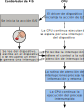
\includegraphics[scale=0.7]{img/ciclo_de_io_por_int.pdf}
    \end{textblock}
\end{frame}

\begin{frame}{Acceso Directo a Memoria (DMA)}
    \begin{textblock}{90}(8,12)
    \small
    Los mecanismos de \texttt{DMA} o Entrada/salida programada (PIO) se ocupan de tomar el control del bus de memoria y realizar las tareas de transferencia de datos que realizaría el procesador.\\
    \medskip
    Para esto se debe contar con un \emph{buffer} en memoria física que utilizará el sistema para dejar los datos que el \texttt{DMA} requiera.\\
    \medskip
    El sistema cuenta con multiples dispositivos \texttt{DMA}, debe coordinar su uso, priorizando las tareas de trasnferencia de datos a realizar.
    % - acceso directo a memoria
    % - scatter-gather
    % - doble buffering
    % - DMA-request DMA-acknowledge
    \begin{enumerate}
    \item El sistema selecciona una tarea de transferencia en la cola de espera del dispositivo \texttt{DMA}.
    \item Configura los registros de control y configuración del \texttt{DMA}.
    \item Queda a la espera de la interrupción de finalización para cargar una nueva tarea de transferencia.
    \end{enumerate}
    \end{textblock}
    \begin{textblock}{100}(105,12)
    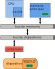
\includegraphics[scale=0.9]{img/dma.pdf}
    \end{textblock}
\end{frame}

\begin{frame}{Tipos de dispositivos de E/S}
    Los dispositivos de E/S son variados, y por lo tanto existen diferentes formas de clasificarlos.\\
    \bigskip
    \begin{tabular}{lp{10cm}}
    \footnotesize \multirow{2}{*}{\textcolor{naranjauca}{Modo de transferencia de datos}}
    & \footnotesize \textbf{Flujo de caracteres}: transfiere de a bytes \textcolor{gray}{(Ej. teclado)} \\
    & \footnotesize \textbf{Flujo de bloques}: transfiere de a bloques de bytes \textcolor{gray}{(Ej. disco)} \vspace{0.2cm} \\
    \pause
    \footnotesize \multirow{2}{*}{\textcolor{naranjauca}{Método de acceso}}
    & \footnotesize \textbf{Acceso secuencial}: acceso es determinado por el dispositivo \textcolor{gray}{(Ej. placa de red)} \\
    & \footnotesize \textbf{Acceso aleatorio}: acceso es determinado por el usuario del dispositivo \textcolor{gray}{(Ej. disco)} \vspace{0.2cm} \\
    \pause
    \footnotesize \multirow{2}{*}{\textcolor{naranjauca}{Forma de transferencia}}
    & \footnotesize \textbf{Síncrona}: el tiempo de respuesta es predecible \textcolor{gray}{(Ej. disco óptico)} \\
    & \footnotesize \textbf{Asíncrona}: el tiempo de respuesta es aleatorio \textcolor{gray}{(Ej. mouse)} \vspace{0.2cm} \\
    \pause
    \footnotesize \multirow{2}{*}{\textcolor{naranjauca}{Compartición}}
    & \footnotesize \textbf{Compartible}: varios procesos lo pueden usar concurrentemente \textcolor{gray}{(Ej. teclado)} \\
    & \footnotesize \textbf{Dedicado}: solo un proceso lo puede usar a la vez \textcolor{gray}{(Ej. impresora)} \vspace{0.2cm} \\
    \pause
    \footnotesize \multirow{2}{*}{\textcolor{naranjauca}{Velocidad}}
    & \footnotesize \textbf{Latencia}, \textbf{tiempo de búsqueda}, \textbf{tasa de transferencia}, etc.\\
    & \footnotesize \textcolor{gray}{(varía según cada dispositivos)} \vspace{0.2cm} \\
    \pause
    \footnotesize \multirow{3}{*}{\textcolor{naranjauca}{Tipo de operación}}
    & \footnotesize \textbf{Solo lectura}  \textcolor{gray}{(Ej. DVD} \\
    & \footnotesize \textbf{Solo escritura}: \textcolor{gray}{(Ej. controladora gráfica)} \\
    & \footnotesize \textbf{Lectura-escritura}: \textcolor{gray}{(Ej. disco)} \\
    \end{tabular}
\end{frame}

\begin{frame}{Subsistema de E/S}
    Cada proceso debe poder comunicarse con los dispositivos que necesita a través del sistema.\\
    \medskip
    Para esto el sistema provee una interfaz que permite abstraer el acceso a los dispositivos en comandos simples, mientras \textbf{oculta el funcionamiento interno} de cada dispositivo.\\
    \medskip
    \begin{center}
    \large
    \begin{tabular}{ccl}  \cline{3-3}
    \textcolor{naranjauca}{Capa 4} & \includegraphics[scale=0.65]{img/subsistema_graficos-layer5.pdf} & Software de E/S de capa de usuario \vspace{0.3cm}\\ \cline{3-3}
    \textcolor{naranjauca}{Capa 3} & \includegraphics[scale=0.65]{img/subsistema_graficos-layer4.pdf} & Software de S.O. independiente del dispositivo \vspace{0.3cm}\\ \cline{3-3}
    \textcolor{naranjauca}{Capa 2} & \includegraphics[scale=0.65]{img/subsistema_graficos-layer3.pdf} & Controladores de dispositivos \vspace{0.3cm}\\ \cline{3-3}
    \textcolor{naranjauca}{Capa 1} & \includegraphics[scale=0.65]{img/subsistema_graficos-layer2.pdf} & Manejadores de interrupciones y rutinas \vspace{0.3cm}\\ \cline{3-3}
    \textcolor{naranjauca}{Capa 0} & \includegraphics[scale=0.65]{img/subsistema_graficos-layer1.pdf} & Hardware \vspace{0.3cm}\\ \cline{3-3}
    \end{tabular}
    \end{center}
\end{frame}

\begin{frame}{Capa 1: Manejador de interrupciones y rutinas}
    \begin{textblock}{140}(115,2) \includegraphics[scale=0.37]{img/subsistema_entrada_salida-layer1.pdf} \end{textblock}
    \begin{textblock}{140}(115,2) \includegraphics[scale=0.37]{img/subsistema_entrada_salida-layer3.pdf} \end{textblock}
    Por medio de un conjunto de rutinas básicas, el sistema operativo\\
    puede \textbf{atender interrupciones} y dar el control a las capas superiores.\\
    \bigskip
    Además utiliza rutinas especiales, que permiten acceder al\\ \textbf{espacio de memoria de los dispositivos}.\\
    \bigskip
    \pause
    El sistema cuenta con todo tipo de rutinas para atender dispositivos, desde\\
    \textbf{rutinas genéricas} para dispositivos, donde solo se provee una interfaz para acceder a memoria,\\
    hasta complejas rutinas para \textbf{atender dispositivos específicos}.\\
    \bigskip
    \textcolor{naranjauca}{El desarrollo de esta capa es fundamental para construir drivers de dispositivo eficientes.}
%     Todos estos pasos consumen muchos ciclos de CPU.\\
%     Primera conclusión: \textcolor{naranjauca}{hacer E/S es costoso para el rendimiento del sistema}.
\end{frame}

\begin{frame}{Capa 2: Controladores de dispositivos (\textit{drivers})}
    \begin{textblock}{140}(115,2) \includegraphics[scale=0.37]{img/subsistema_entrada_salida-layer1.pdf} \end{textblock}
    \begin{textblock}{140}(115,2) \includegraphics[scale=0.37]{img/subsistema_entrada_salida-layer4.pdf} \end{textblock}
    El funcionamiento de cada dispositivo depende del fabricante.\\
    Este implementa un \textbf{protocolo de comunicación particular}.\\
    \bigskip
    Para esto, los fabricantes proveen \textbf{\emph{drivers}} específicos para cada\\
    dispositivo y sistema donde serán utilizados.\\
    \bigskip
    \textcolor{naranjauca}{La interfaz de la capa anterior es utilizada por los \emph{drivers} para acceder directamente al hardware.\\}
    \pause
    \bigskip
    \textcolor{gray}{Por esta razón, muchas veces los sistemas no implementan las interfaces que necesitan los drivers, y por lo tanto son incompatibles con el sistema.
    Otras veces, los fabricantes directamente no dan soporte para algunos sistemas operativos.}\\
    \bigskip
    Los \textit{drivers} deben ser rutinas \textcolor{naranjauca}{\textbf{reentrantes}}, es decir que deben poder recibir una nueva solicitud mientras están ejecutando otra.
\end{frame}

\begin{frame}{Capa 3: Subsistema de E/S independiente del dispositivo}
    \begin{textblock}{140}(115,2) \includegraphics[scale=0.37]{img/subsistema_entrada_salida-layer1.pdf} \end{textblock}
    \begin{textblock}{140}(115,2) \includegraphics[scale=0.37]{img/subsistema_entrada_salida-layer5.pdf} \end{textblock}
    \vspace{0.5cm}
    Publica una \textbf{interfaz uniforme} para acceder a los dispositivos.\\
    \medskip
    Los \emph{drivers} se deben adaptar y exponer la interfaz que el sistema propone.\\
    De esta forma todos los dispositivos de comportamiento similar,\\
    son utilizandos por los usuarios de la misma forma.\\
    \textcolor{gray}{Ej. disco óptico, disco rígido, disco de estado sólido}\\
    \pause
    \bigskip
    Además se ocupa de la \textbf{Planificación de E/S}.\\
    \medskip
    Determinando el orden en que se atenderán las solicitudes\\
    y respetando las prioridades entre los diferentes dispositivos.\\
    \bigskip
    Esta capa también se ocupa de resolver las \textbf{operaciones comunes} a todos los dispositivos
\end{frame}

\begin{frame}{Capa 3: Subsistema de E/S independiente del dispositivo}
    \begin{textblock}{140}(115,2) \includegraphics[scale=0.37]{img/subsistema_entrada_salida-layer1.pdf} \end{textblock}
    \begin{textblock}{140}(115,2) \includegraphics[scale=0.37]{img/subsistema_entrada_salida-layer5.pdf} \end{textblock}
    Algunas de las operaciones comunes que resuelve esta capa:\\
    \bigskip
    \small
    \textcolor{naranjauca}{Administración de búferes}\\
    Los datos a transferir se almacenan temporalmente en memoria, permitiendo adaptar los tamaños de transferencia entre dispositivos y sistema.\\
    \bigskip
    \pause
    \textcolor{naranjauca}{Administración de errores}\\
    Los errores son capturados poer el sistema como resultado de una operación de E/S.
    Existen errores que pueden dejar al sistema en un estado inconsistente que debe ser administrado correctamente para evitar la perdida de datos.\\
    \bigskip
    \pause
    \textcolor{naranjauca}{Asignación y liberación de dispositivos dedicados}\\
    El sistema debe aceptar y rechazar solicitudes de uso de dispositivos teniendo en cuenta las características de uso de cada uno.
    Evitando en todo momento generar \emph{deadlocks} por condiciones de sincronización.
\end{frame}

\begin{frame}{Capa 4: Software de E/S en la capa de usuario}
    \begin{textblock}{140}(115,2) \includegraphics[scale=0.37]{img/subsistema_entrada_salida-layer1.pdf} \end{textblock}
    \begin{textblock}{140}(115,2) \includegraphics[scale=0.37]{img/subsistema_entrada_salida-layer6.pdf} \end{textblock}
    Esta capa esta formada por el conjunto de \textbf{bibliotecas de funciones}\\
    que resuelven el acceso a E/S:\\
    \bigskip
    Proporcionan comandos o funciones que nos permiten utilizar los recursos que proveen los dispositivos de forma más simple.\\
    \bigskip
    \small
    \textcolor{gray}{Por ejemplo, la función \texttt{printf} que se utiliza para imprimir en pantalla,
    lama internamente a \emph{syscalls} como \texttt{write} cuando se debe imprimir un texto largo o \texttt{put} cuando se debe imprimir un solo caracter.}\\
    \medskip
    \textcolor{gray}{Mientras tanto, \texttt{open} y \emph{close} son funciones que se pueden utilizar para abrir y cerrar archivos o dispositivos de caracteres mapeados archivos.}\\
    \medskip
    \textcolor{gray}{Otro ejemplo es \texttt{write} que puede ser utilizada como \emph{syscall} para imprimir en pantalla o para imprimir dentro de un archivo, incluso información binaria.}\\
\end{frame}

\begin{frame}{Relojes}
    \small
    Los relojes son un tipo específico de dipositivo de entrada/salida.\\
    \medskip
    Su interfaz de hardware se ocupa de \textbf{generar eventos en intervalos regulares de tiempo}.\\
    Estos eventos se suelen traducir en interrupciones o dejan registro en contadores.\\
    \medskip
    \textcolor{naranjauca}{\textbf{Los sistemas cuentan con múltiples relojes que operan a distintas frecuencias}}\\
    \medskip
    El sistema distingue entre distintas fuentes de tiempo:
    \begin{itemize}
    \setlength\itemsep{0cm}
    \item[$\cdot$] Temporizador de tiempo real (\emph{real-time-clock}, \texttt{RTC}).
    \item[$\cdot$] Temporizador de eventos de alta precisión (\emph{high precision event timer}, \texttt{HPET})
    \end{itemize}
    La interfaz del reloj provee tres funciones básicas:\\
    \begin{itemize}
    \setlength\itemsep{0cm}
    \item[-] Obtener el tiempo actual.
    \item[-] Obtener el tiempo transcurrido desde el último evento.
    \item[-] Configurar el reloj para despertar la operación X en el momento T.
    \end{itemize}
    \textcolor{verdeuca}{
    Internamente el sistema requiere múltiples relojes, para resolver esto, se crean \textbf{relojes virtuales}.\\
    Los relojes virtuales se actualizan o cambian su estado en función de los relojes físicos.}
\end{frame}

\begin{frame}{Administración de energía}
    \small
    El sistema operativo juega un rol fundamental en la administración de la energía.\\
    \medskip
    Ya sea que se cuente con una bateria como fuente de alimentación o se esté conectado a la red eléctrica.
    \textcolor{naranjauca}{La \textbf{reducción del consumo} de energía es un eje básico de diseño.}\\
    \medskip
    \textcolor{verdeuca}{Los sistemas están diseñados para disipar una determinada cantidad de energía que se manifiesta en \textbf{calor}.
    Este calor debe ser reducido mediante sistemas de enfriamiento como \emph{coolers}.}
    \medskip
    \begin{tcolorbox}[size=small,width=\textwidth,colback={gray!30},title={\emph{Advanced Configuration and Power Interface} (\texttt{ACPI})}]
    \small
    Provee un estándar para que el sistema operativo pueda descubrir y configurar los componentes de hardware del sistema y administrar el consumo de energía.
    Permite monitorar el uso del los componentes, su estado, y mecanismos de \emph{Plug and Play} y \emph{hot swapping}.
    \end{tcolorbox}
    \medskip
    \textcolor{verdeuca}{El sistema operativo se encarga de decidir cuando \textbf{encender o apagar componentes},\\
    o incluso \textbf{degradar su funcionamiento} para reducir el consumo.}\\
    \medskip
    \textcolor{naranjauca}{Esta tarea es muy compleja ya que para reducir el consumo se debe \textbf{afectar la experiencia de usuario.}}
\end{frame}

\begin{frame}{Almacenamiento Masivo - Tecnologías de discos}
    Existen distintos tipos de tecnologías de almacenamiento secundario.\\
    \bigskip
    \textcolor{naranjauca}{\textbf{Discos magnéticos}} o \textcolor{naranjauca}{\textbf{HDDs}} (\textit{Hard Disk Drives}).\\
    Está compuestos por discos recubiertos de material magnético que giran a una velocidad de entre 5400 a 15000 RPM.
    Sobre estos discos un brazo se posiciona y escribe o lee información.
    % Velocidad de transferencia (transfer rate)
    % Velocidad de posicionamiento (positioning time)
    % Tiempo de búsqueda (seek time)
    % Latenia rotacional (rotational latency)
    \bigskip
    \textcolor{naranjauca}{\textbf{Discos de estado sólido}} o \textcolor{naranjauca}{\textbf{SSDs}} (\textit{Solid-State Drives}).\\
    Son un arreglo de memorias tipo \texttt{flash}, que para evitar el desgaste por reiteradas escrituras cuentan con una capa de traducción.
    Esta capa virtualiza el espacio de escritura, permitiendo que todas las escrituras nuevas se realicen sobre bloques diferentes del disco.
    % máxima cantidad de escrituras
    % distribuir uniformemente las escrituras
    % write amplification
    \bigskip
    \textcolor{naranjauca}{\textbf{Discos de RAM}} o \textcolor{naranjauca}{\textbf{RAMdisk}} (\textit{RAM Disk Drives}).\\
    Se implementan por medio de placas conectadas directamente al bus de entrada/salida. Estas placas son un arreglo de memorias tipo RAM.
    Si bien lo consideramos un tipo de disco, porque se utiliza como interfaz, su almacenamiento es volatil, a diferencia de los anteriores.
\end{frame}

\begin{frame}{Formateo de bajo nivel}
    Inicialmente los discos no tienen ningún formato específico.\\
    Ni siquiera cuentan con la construcción lógica de un sector.\\
    Parar esto se realiza el \textbf{formateo de bajo nivel}.\\
    \medskip
    \begin{center}
    \begin{tabular}{|c|c|c|}
    \hline
    Encabezado & \ \ \ \ \ \ \ \ \ \ \ \ \ \ ... Datos ... \ \ \ \ \ \ \ \ \ \ \ \ \ \ & Código de correción de errores\\
    \hline
    \end{tabular}
    \end{center}
    \bigskip
    Consiste en construir una estructura con información del sector y disco, datos e información para la correción de errores.
    Esta última, permite no solo detectar, sino arreglar errores que puedan tener los datos.\\
    \medskip
    \textcolor{verdeuca}{El tamaño de los datos para un sector puede ser de entre 512 bytes a 4KB.\\}
\end{frame}

\begin{frame}{Particiones en un disco}
    Los discos suelen ser particionados tanto para ordenar la información, como por razones funcionales.
    Cada partición puede contener un determinado sistema de archivos o datos \emph{raw}.\\
    \bigskip
    \textcolor{gray}{Algunas aplicaciones especiales como los motores de bases de datos o el espacio de intercambio (\emph{swap}) no necesitan un formato especial.}\\
    \bigskip
    \textcolor{naranjauca}{\textbf{Particiones}}\\
    Las particiones que se utilizarán para sistemas de archivos, se formatean escribiendo conjuntos de sectores la \emph{metadata} que permite determinar donde se guarda cada archivo.
    \bigskip
    % Editor de particiones
    \textcolor{naranjauca}{\textbf{Sector de arranque}} o \textcolor{naranjauca}{MBR (\textit{Master-boot Record})}\\
    Es un sector distingido del disco que almacena datos sobre la tabla de particionado y rutinas de código básicas que sirven como el primer paso en la carga del sistema operativo.
    % FIGURA boot-loader del MBR
\end{frame}

%     RAID (Arreglo Redundante de Discos Económicos)

\begin{frame}[fragile]
    \frametitle{Bibliografía}
    \begin{itemize}
        \setlength\itemsep{0.5cm}
        \item[-] \small Silberschatz, ``Fundamentos de Sistemas Operativos'', 7ma Edición, 2006.\\
        \begin{itemize}
            \item \textbf{Capítulo 13 - Sistema de E/S}
            \begin{itemize}
                \item 13.3 Interfaz de E/S de las aplicaciones
                \item 13.4 Subsistema de E/S del kernel
%                \item 13.5 Transformación de las solicitudes de E/S en operaciones hardware
%                \item 13.7 Rendimiento
            \end{itemize}
            \item \textbf{Chapter 11 - Mass-Storage Structure}, páginas 452-454 y 461-462
        \end{itemize}
        \item[-] \small Tanenbaum, ``Modern Operating Systems'', 4th Edition, 2015.\\
        \begin{itemize}
            \item \textbf{Chapter 5 - Input/Output}
            \begin{itemize}
                \item 5.2 Principles of I/O software
                \item 5.3 I/O software layers
                \item 5.5 Clocks
                \item 5.8 Power management
            \end{itemize}
        \end{itemize}
        \item[-] \small Silberschatz, ``Fundamentos de Sistemas Operativos'', 7ma Edición, 2006.\\
        \begin{itemize}
            \item \textbf{Capítulo 12 - Estructura de almacenamiento masivo}, páginas 407-410 y 412-423
        \end{itemize}
    \end{itemize}
\end{frame}

\begin{frame}[plain]
    \begin{center}
    \vspace{2cm}
    \huge ¡Gracias!\\
    \vspace{2cm}
    \normalsize Recuerden leer los comentarios adjuntos\\ en cada clase por aclaraciones.
    \end{center}
\end{frame}

\end{document}
